\section{Data, representations, and empirical design}\label{sec:design}

Chart construction combines local high--low scaling, a binary grayscale image, and flexible learning. We examine these components through a controlled representation comparison. The logistic models show how scaling affects the stock ranking within a fixed linear architecture before nonlinear learning is added. The chart CNN and CNN1D then receive the same locally scaled market history, and the multimodal model tests whether their representations contain complementary predictive information. We hold timing, ranking, weighting, and transaction-cost rules fixed across the learned scores.

\subsection{Sample and prediction target}\label{subsec:sample}

To hold the data environment fixed, we construct a daily CRSP panel of ordinary common shares listed on NYSE, AMEX, or Nasdaq using share codes 10 and 11. The panel includes daily returns, open, high, low, and close prices, trading volume, lagged market capitalization, stock identifiers, and available delisting returns. At each formation date, eligibility requires positive prices and sufficient history for the relevant signal. Firms enter and leave with their CRSP histories, producing an unbalanced panel with no survivorship requirement.

We separate model development from economic evaluation. Model development uses data from 1993--2000, and all portfolio results are evaluated out of sample from 2001 to 2024. We report the full evaluation period, a 2001--2019 baseline sample, and a 2020--2024 extension sample.

Our model grid combines 5-, 20-, and 60-day input windows with 5-, 20-, and 60-day forecast horizons. We write each specification as $I/R$, so $I20/R5$ uses 20 trading days of market history to predict the return sign over the next five trading days. For stock $i$ at formation date $t$, the directional target is defined by
\begin{equation}
 y_{i,t}^{(R)}=\mathbbm{1}\!\left(\prod_{j=1}^{R}(1+r_{i,t+j})-1>0\right).
 \label{eq:label}
\end{equation}
The target period begins at $t+1$, after all input information has been observed by the close of date $t$.

Stock splits can create jumps in raw nominal prices even when the underlying return path is continuous. We therefore set the first close in each input window to one, reconstruct subsequent closes from daily returns, and scale open, high, and low prices consistently with the reconstructed close series. The moving-average window equals $I$. The chart and sequence inputs are constructed from this common price-consistent market history and trading volume.

Within each specification, the three learned models use the same underlying data. Eligible cross-sections can vary across input windows and price-based benchmarks because the signals require different amounts of historical data. Each portfolio uses the sample available for its signal under common portfolio rules. Direct comparisons of the chart CNN, CNN1D, and multimodal scores use an exact common stock-date sample. Portfolio performance and signal overlap are therefore evaluated on samples suited to their distinct questions.

\subsection{From market histories to charts}\label{subsec:representation_design}

The chart input combines local scaling with a binary grayscale representation. Local scaling removes nominal price levels and preserves the relative shape and range of each stock's recent path. Chart construction then places open, high, low, close, moving-average, and volume information in a fixed image layout processed by the chart CNN. We use the representation tests to assess the contribution of local scaling and the chart image.

For each stock and formation date, we scale the five price channels within the lookback window. Let $m_{i,t}^{(I)}$ and $M_{i,t}^{(I)}$ denote the minimum and maximum calculated jointly across all open, high, low, close, and moving-average observations in that window. Each price-channel observation $x_{i,t-j}$ is then transformed using these values,
\begin{equation}
 \widetilde{x}_{i,t-j}
 =\frac{x_{i,t-j}-m_{i,t}^{(I)}}{M_{i,t}^{(I)}-m_{i,t}^{(I)}}.
 \label{eq:image_scale}
\end{equation}
Trading volume is min--max scaled separately within the same window.

After scaling, we construct the chart using daily OHLC bars, a moving-average line, and a separate lower panel for trading volume. The 5-, 20-, and 60-day images have dimensions $32\times15$, $64\times60$, and $96\times180$ pixels. Pixels corresponding to the OHLC bars, moving-average line, and volume bars take value one, while empty pixels take value zero. The resulting binary grayscale image in Figure~\ref{fig:chart_input_transformation} preserves the relative structure of recent prices and volume.

\begin{figure}[htbp]
\centering
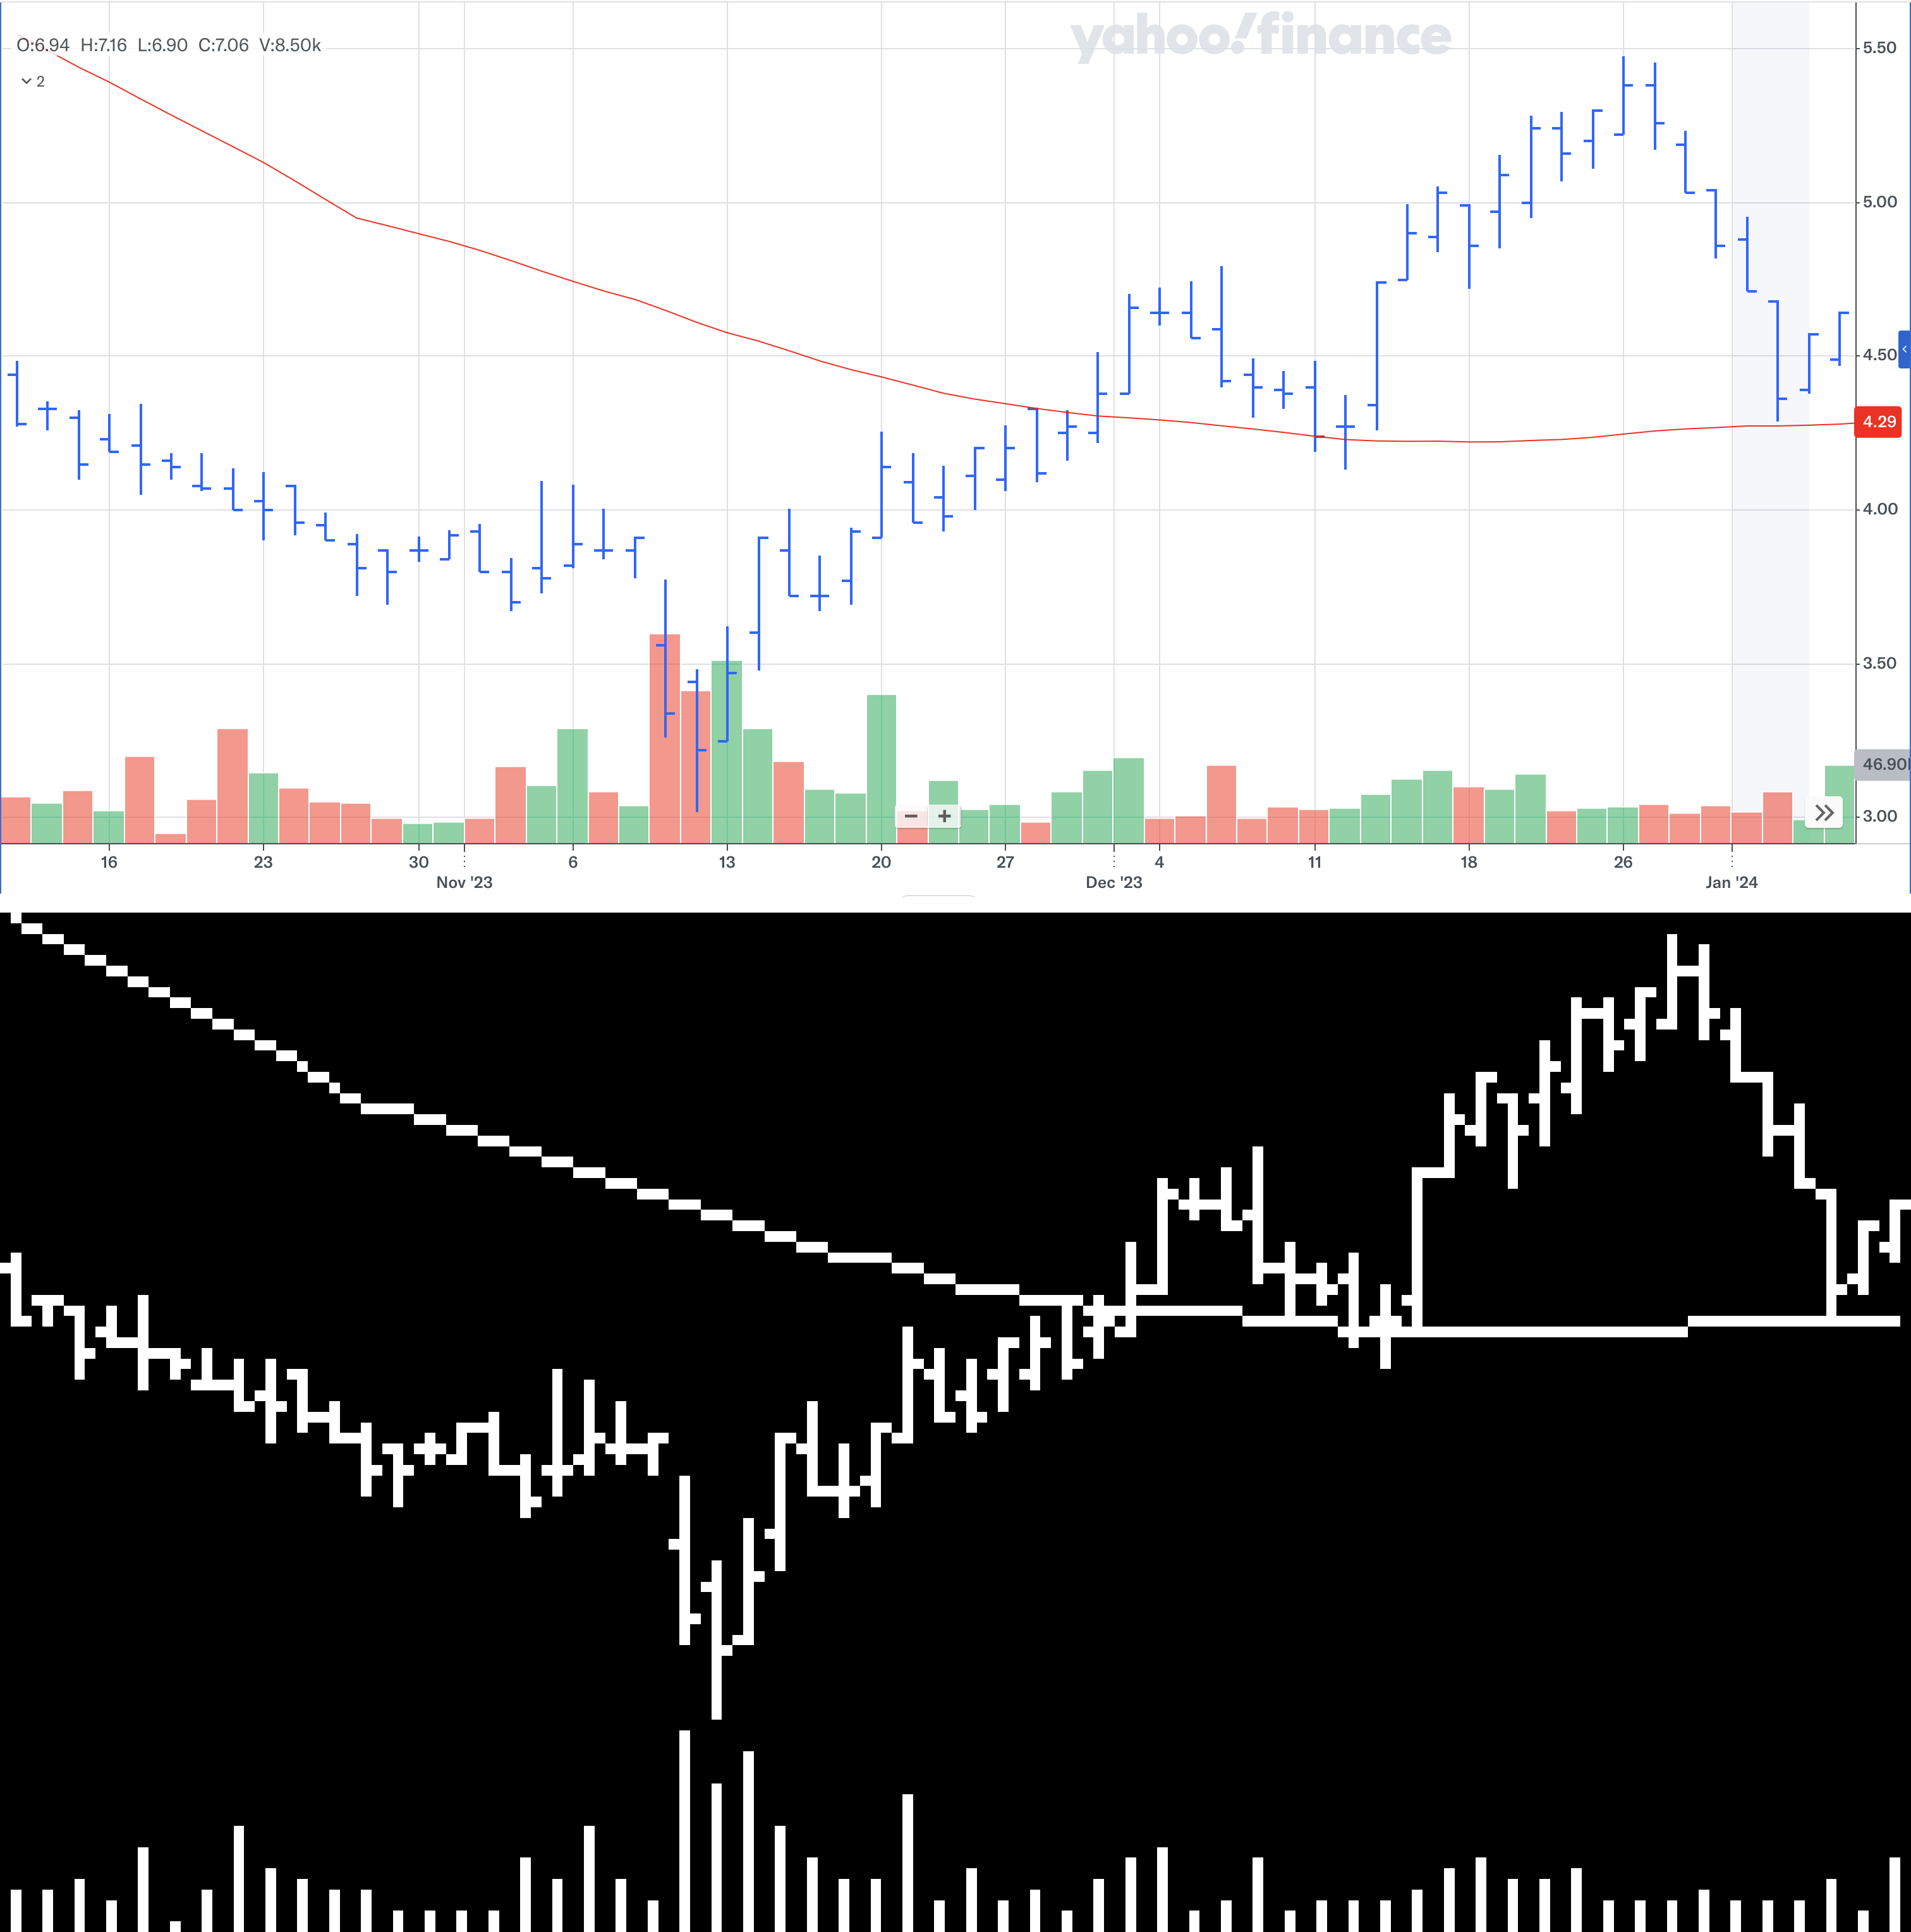
\includegraphics[width=0.82\textwidth,height=0.78\textheight,keepaspectratio]{chart_input_transformation.png}
\caption{Example of chart construction and model input. The upper panel shows a conventional 60-day OHLC chart for Envela Corporation (ELA). The lower panel shows the corresponding binary grayscale image used by the chart CNN, with the OHLC bars and moving-average line in the price panel and trading volume in the lower panel.}
\label{fig:chart_input_transformation}
\end{figure}

Each sequence observation contains six aligned daily series in chronological order. The channels are open, high, low, close, moving average, and trading volume. We evaluate the image scale, cumulative-return scale, and devolatized-return scale. Under image scaling, the price channels retain the continuous within-window values from Eq.~\eqref{eq:image_scale}, while volume is scaled separately. The cumulative-return scale anchors each price channel to the first close in the lookback window. The devolatized-return scale expresses price changes relative to lagged exponentially weighted volatility and volume through relative changes. We standardize each transformed channel using development-sample means and standard deviations that remain fixed throughout the evaluation period.

The chart and image-scaled sequence use the same local normalization. The sequence retains continuous open, high, low, close, moving-average, and volume observations as channels ordered by trading day. The chart converts these observations into a fixed binary pixel layout, which reduces numerical precision while preserving relative shape and location. The image-scaled sequence therefore shows how much of the chart CNN's stock ranking can be reproduced from the same locally scaled market history.

Table~\ref{tab:design_map} summarizes the model inputs, scaling schemes, and model structures used in the representation comparison. The logistic classifiers use the scaled sequence inputs as linear indices and show how much predictive content each scaling scheme makes available to a linear model. CNN1D learns nonlinear temporal patterns from the same numerical channels. The chart CNN learns from the binary grayscale image, and the multimodal model combines the chart and sequence representations through paired branches.

The logistic specifications use the same directional target as CNN1D and map the flattened sequence into a linear index. Comparing them across scaling schemes measures how scaling changes the ranking within a fixed linear model. Comparing logistic and CNN1D under local scaling measures the increment associated with nonlinear interactions across adjacent observations. The chart CNN/CNN1D comparison then asks whether the binary image representation produces an economically different ranking after both models receive the same locally normalized history.

The final comparison studies complementarity. Multimodal inputs are paired by stock, formation date, input interval, and forecast horizon. A stable improvement from fusion would show that the chart and sequence branches extract differences that are useful in the portfolio sort. Similar branch and fusion performance would point toward a common economic signal. This evidence is descriptive because the fusion rule and optimization can constrain the joint model. The central interpretation therefore rests on patterns that recur across scaling schemes, input windows, model specifications, and the separate overlap tests.

The design narrows the source of performance without creating a pure treatment for layout. Chart and sequence models differ in numerical precision, dimensionality, filter geometry, depth, and capacity. We interpret similar performance after local scaling as evidence that the pixel image is unnecessary for reproducing the tested ranking. Residual differences can arise from any of the remaining representation or architecture features.

\begin{table}[htbp]
\centering
\caption{Models and scaling schemes in the representation comparison}
\label{tab:design_map}
\small
\renewcommand{\arraystretch}{1.06}
\begin{tabularx}{\textwidth}{@{}>{\raggedright\arraybackslash}p{0.21\textwidth}>{\raggedright\arraybackslash}p{0.23\textwidth}>{\raggedright\arraybackslash}p{0.25\textwidth}L@{}}
\toprule
Model & Scaling & Input representation & Model structure \\
\midrule
Logistic classifier & Cumulative-return scale & Continuous sequence & Linear logit \\
Logistic classifier & Devolatized-return scale & Continuous sequence & Linear logit \\
Logistic classifier & Image scale & Continuous sequence & Linear logit \\
CNN1D & Cumulative-return scale & Continuous sequence & Temporal convolution \\
CNN1D & Devolatized-return scale & Continuous sequence & Temporal convolution \\
CNN1D & Image scale & Continuous sequence & Temporal convolution \\
Chart CNN & Image scale & Binary grayscale image & Two-dimensional convolution \\
Multimodal model & Image scale & Chart and sequence & Paired branches with fusion \\
\bottomrule
\end{tabularx}
\end{table}

\FloatBarrier

\subsection{Prediction models and estimation}\label{subsec:models}

The chart CNN architecture follows the design used by \textcite{reimagining_price_trends_jiang}. We estimate separate variants for the 5-, 20-, and 60-day chart inputs. Their depth increases with the length and resolution of the input image, with two, three, and four convolutional blocks, respectively. Each block applies a $5\times3$ convolution, batch normalization, Leaky ReLU activation, and max pooling. The final feature map is flattened, dropout is applied, and a fully connected layer maps the learned representation to the two return-sign classes.

We estimate separate CNN1D architectures for the 5-, 20-, and 60-day sequence inputs. Each block applies a one-dimensional convolution along the time dimension, followed by the same normalization, activation, and pooling operations as in the chart CNN. The filters span three trading days and observe all six channels at each location. The three input lengths use one, two, and three blocks, respectively. The first block has 64 output channels, and the channel count doubles in each subsequent block. After flattening, the final sequence representation passes through the same dropout and fully connected classification layers as the chart CNN.

Each multimodal observation pairs a chart image and a sequence input for the same stock, formation date, input interval, and forecast horizon. The chart CNN and CNN1D branches process their inputs separately. Let $f^{2D}_{i,t}$ and $f^{1D}_{i,t}$ denote the corresponding feature vectors. Feature concatenation forms the joint representation
\begin{equation}
 f^{MM}_{i,t}=\left[f^{2D}_{i,t};f^{1D}_{i,t}\right].
 \label{eq:fusion}
\end{equation}
The concatenated feature vector is passed to a linear classifier and the final softmax layer. This design allows each branch to learn its own representation before the classifier combines them. We also examine late fusion, where the chart CNN and CNN1D produce separate predictions that are combined through probability or logit averaging. Comparing the multimodal and single-branch models tests whether the two representations contain complementary predictive information.

The final layer of each model produces one score for the down class and one for the up class. The softmax transformation converts these scores into probabilities. The probability assigned to the up class is
\begin{equation}
 s_{i,t}=\frac{\exp(z_{i,t}^{(1)})}
 {\exp(z_{i,t}^{(0)})+\exp(z_{i,t}^{(1)})},
 \label{eq:score}
\end{equation}
We carry $s_{i,t}$ forward as a within-date ranking score for the portfolio analysis. We do not interpret it as a calibrated expected return.

All learned model families are estimated within a common prediction framework. We estimate separate models across input intervals, forecast horizons, model families, and, where applicable, sequence scaling or fusion design. The neural models use cross-entropy loss, the Adam optimizer, a learning rate of $10^{-4}$, a batch size of 128, dropout probability of 0.50, Xavier initialization, and a maximum of 50 training epochs.

Training stops when validation loss does not improve for two consecutive epochs. We retain the model parameters from the epoch with the lowest validation loss as the selected checkpoint. These parameters remain fixed throughout the 2001--2024 evaluation period and produce one up-class probability for each eligible stock-date observation.

Model development uses data from 1993--2000. We randomly divide stock-date observations into 70\% training and 30\% validation sets using a fixed seed. Observations from the same firm or calendar period can therefore appear in both sets. Validation is used to select the checkpoint within the pre-2001 development sample. Portfolio evaluation begins in 2001, after model fitting and checkpoint selection are complete.

The main analysis uses one selected checkpoint for each learned specification. The portfolio score is therefore the single-model up-class probability from that checkpoint. For $I5/R5$ and $I20/R5$, the online appendix compares the single-model chart CNN with matched five-member forecast averages. This sensitivity check is limited to these weekly chart CNN specifications, and the weekly conclusions remain unchanged.

\subsection{Portfolio construction}\label{subsec:portfolios}

At each formation date, stocks are sorted according to the relevant model score or benchmark signal, and the eligible cross-section is divided into ten deciles. The high-minus-low portfolio buys the highest-score decile and shorts the lowest-score decile. We report equal-weighted and value-weighted portfolios. Equal weighting assigns the same weight to each stock within a leg, while value weighting uses lagged market capitalization normalized separately within the long and short legs. Each leg carries one dollar of notional, so the spread has zero net investment and two dollars of gross exposure.

Weekly, monthly, and quarterly portfolios correspond to the 5-, 20-, and 60-trading-day forecast horizons. At formation date $t$, the model score uses information available through the close of that date and ranks stocks for the return from $t+1$ through $t+R$. We use one formation date per holding interval, producing non-overlapping return series at each evaluation frequency. For a portfolio return series $R_{p,t}$ with $K\in\{52,12,4\}$ observations per year, the reported Sharpe ratio is
\begin{equation}
 \mathrm{SR}_{p}=\sqrt{K}\,\frac{\overline{R}_{p}}{\operatorname{sd}(R_{p,t})}.
 \label{eq:sharpe}
\end{equation}
No risk-free rate is subtracted from the zero-net-investment spread.

Benchmark signals can require longer histories than the learned models, which produces different eligible cross-sections. All methods use common ranking, horizon, weighting, and transaction-cost rules within the same CRSP universe. Comparisons among the chart CNN, CNN1D, and multimodal model use the exact common stock-date sample described in Section~\ref{subsec:sample}.

We report the complete grid across input intervals and forecast horizons. Later figures and economic tests use $I20/R5$ as the representative weekly specification. It is central to the short-horizon grid, performs strongly across all three learned model families, and allows the models to be compared under the same horizon structure. We selected this specification after examining the grid, so the focused results are descriptive.

\subsection{Price-based benchmarks}\label{subsec:benchmarks}

We compare the learned models with four transparent price-based benchmark strategies. These are momentum (MOM), one-month short-term reversal (STR), one-week short-term reversal (WSTR), and the multi-horizon trend strategy (TREND). MOM captures continuation, STR and WSTR capture reversal at different horizons, and TREND captures broader multi-horizon trend information. All four strategies are evaluated under the common portfolio rules described above.

MOM is the medium-horizon continuation benchmark. Following \textcite{jegadeeshReturnsBuyingWinners1993a}, we implement a daily analogue of a 12--1 momentum strategy. The signal is the cumulative return over the previous 252 trading days, excluding the most recent 21 trading days,
\begin{equation}
 z^{\mathrm{MOM}}_{i,t}=\prod_{j=22}^{273}(1+r_{i,t-j})-1.
 \label{eq:mom}
\end{equation}
The exclusion of the most recent 21 trading days separates medium-horizon continuation from the short-term reversal patterns captured by STR and WSTR.

One-month short-term reversal (STR) follows \textcite{jegadeeshEvidencePredictableBehavior1990} and uses the negative of the previous 21-trading-day return. One-week short-term reversal (WSTR) follows \textcite{lehmannFadsMartingalesMarket1990} and uses the negative of the previous 5-trading-day return.
\begin{equation}
 z^{\mathrm{STR}}_{i,t}=-\left(\frac{P_{i,t}}{P_{i,t-21}}-1\right),
 \qquad
 z^{\mathrm{WSTR}}_{i,t}=-\left(\frac{P_{i,t}}{P_{i,t-5}}-1\right).
 \label{eq:reversal}
\end{equation}
High scores identify recent losers. The price series used for both signals is split-consistent with the return history. WSTR provides the closest transparent benchmark to the learned weekly forecast horizon.

TREND follows the multi-horizon trend strategy of \textcite{hanTrendFactorAny2016} and combines moving-average information across several horizons. For each lag $L$ in the set
\[
 \mathcal{L}=\{3,5,10,20,50,100,200,400,600,800,1000\}
\]
we define $x_{i,t,L}=\mathrm{MA}_{i,t,L}/P_{i,t}$, which compares the moving average with the current price. At each formation date, a cross-sectional regression maps these signals into next-period returns. The forecasting coefficients are the trailing mean of the previous 12 fully realized coefficient vectors. The date-$t$ TREND score is
\begin{equation}
 z^{\mathrm{TREND}}_{i,t}=\sum_{L\in\mathcal{L}}\overline{\beta}_{L,t}x_{i,t,L}.
 \label{eq:trend}
\end{equation}
TREND is a supervised linear benchmark with explicit features and lagged coefficient estimation.

\subsection{Cost adjustment and implementation tests}\label{subsec:economic_tests}

We report both gross and net portfolio performance. At each rebalancing date, turnover for each leg is measured from the change between its previous and target portfolio weights. For $\ell\in\{\mathrm{long},\mathrm{short}\}$, turnover is
\begin{equation}
 \mathrm{Turnover}^{\ell}_{t}=\frac{1}{2}\sum_i
 \left|w^{\ell,\mathrm{target}}_{i,t}-w^{\ell,\mathrm{prev}}_{i,t}\right|.
 \label{eq:turnover}
\end{equation}
Total turnover is the sum of turnover in the long and short legs and is reported as a monthly-equivalent average. Net performance applies a one-way transaction cost to the full absolute traded notional in both portfolio legs. This traded notional equals twice the conventional half-turnover measure used for reported turnover. Stocks above the contemporaneous NYSE 80th-percentile market-cap breakpoint are charged 10 basis points, while the remaining stocks are charged 20 basis points. Net return is
\begin{equation}
 R^{\mathrm{net}}_{p,t}=R^{\mathrm{gross}}_{p,t}
 -\sum_{i,\ell}c_{i,t}\left|\Delta w^{\ell}_{i,t}\right|.
 \label{eq:netreturn}
\end{equation}
The common cost schedule provides a transparent implementation test. It does not account for stock-specific spreads, price impact, borrowing costs, short-sale constraints, or capacity limits.

We re-form the representative $I20/R5$ weekly portfolios under five tradability screens. The screens require a closing price of at least \$5, dollar volume of at least \$1 million or \$5 million, market capitalization above the NYSE 20th-percentile breakpoint, or the combined price, \$5 million dollar-volume, and market-capitalization conditions. Dollar volume equals closing price times trading volume at the formation date. The tests use the same saved model scores as the main analysis and leave the model parameters fixed.

We obtain daily market, size, and value factors and the daily momentum factor from the Kenneth R. French Data Library. Each factor is compounded over the weekly holding interval. We then estimate Carhart four-factor regressions for weekly net high-minus-low returns \parencite{carhartPersistenceMutualFund1997}. The intercepts are annualized, and inference uses Newey--West standard errors with four lags.

\subsection{Signal overlap and conditional content}\label{subsec:overlap_methods}

The portfolio tests show whether the models produce economically useful rankings. We also examine whether the learned-model rankings contain distinct information. For each input interval and forecast horizon, we form an exact common stock-date panel on which all three learned-model scores and future returns are observed. We compute date-level Spearman rank correlations \parencite{spearmanProofMeasurementAssociation1904} and average them through time. These rank correlations compare the full cross-sectional orderings produced by the models.

The second diagnostic asks which learned-model scores retain predictive content when they are observed jointly. At each formation date, we estimate a cross-sectional regression of future returns on all three scores using the exact common stock-date panel \parencite{famaRiskReturnEquilibrium1973},
\begin{equation}
 R_{i,t+1:t+R}=\alpha_t+\beta^{2D}_t s^{2D}_{i,t}
 +\beta^{1D}_t s^{1D}_{i,t}+\beta^{MM}_t s^{MM}_{i,t}
 +\varepsilon_{i,t+R}.
 \label{eq:joint_fmb}
\end{equation}
The Fama--MacBeth coefficients are the time-series averages of the date-level slopes. The conventional test statistics use the time-series standard errors of these slopes without an autocorrelation correction. We therefore treat the significance levels as exploratory, particularly at longer horizons.

A positive coefficient in the joint regression indicates that the corresponding model score contains predictive variation that is not fully absorbed by the other learned-model scores. The regression provides an incremental-content diagnostic within the exact common stock-date panel. Because the scores are up-class probabilities from separately trained models, their numerical scales can differ, and correlation among the scores can affect the coefficient magnitudes. We therefore focus on coefficient signs and patterns that recur across specifications. Rank correlations and portfolio sorts provide the direct evidence on ranking similarity and economic performance.

The model grid contains related comparisons across input intervals, forecast horizons, scaling schemes, model architectures, fusion designs, weighting schemes, and sample periods. We selected the representative $I20/R5$ specification after examining the grid and do not apply a formal multiple-testing correction. We therefore base the interpretation on patterns that recur across the grid and on the separate benchmark, transaction-cost, tradability, and extension-sample evidence. The encompassing regressions provide exploratory evidence on conditional predictive content.
